
% ==================================================
%	Auswertung
% ==================================================

\section{Auswertung}

% ==================================================
%	Stabilitätsbedingung
% ==================================================
\subsection{Stabilitätsbedingung}
\label{sec:Stabilitätsbedingung}

In diesem Versuchteil wurde für zwei Resonatoren der Diodenstrom $I$ in
Abhängigkeit der Resonatorlänge $l$ zur Überprüfung der
Stabilitätsbedingung %TODO
aufgenommen. Hierfür wurde zum einen ein Resonator mit den Spiegelradien
$r_1 = r_2 = \SI{1400}{\mm}$ (bezeichnet mit R1)
und zum anderen ein Resonator mit den
Spiegelradien $r_1 = \SI{1000}{\mm}$ und $r_2 = \SI{1400}{\mm}$
(bezeichnet mit R2) verwandt.
Die zu den Resonatorlängen gemessenen Ströme befinden sich in Tabelle
\ref{tab:S1} und \ref{tab:S2}.
In Abbildung \ref{fig:S1} ist die theoretische Kurve der Stabilitätsbedingung
\ref{eq:Resonanzbedingung} und die gemessenen Ströme für R1 geplottet.
Zu sehen ist in Abbildung \ref{fig:S1}, dass das Minium der theoretischen Kurve
bei $\SI{140}{\cm}$ auch experimentell verifiziert werden kann.
In Abbildung \ref{fig:S2} sind die theoretische Kurve der Stabilitätsbedingung
und die Werte aus Tabelle \ref{tab:S2} dargestellt.
Hier ist ebenfalls zu sehen, dass in dem Bereich wo $g_1g_2 < 0$ ist, auch der
Laser nicht gearbeitet hat und demzufolge kein Strom gemessen wird.

\begin{table}
	\centering
	\begin{tabular}{cc|cc|cc}
		\midrule
		\midrule
		$l/\si{\cm}$ & $I/\si{\mA}$ & $l/\si{\cm}$ & $I/\si{\mA}$ &
		$l/\si{\cm}$ & $I/\si{\mA}$ \\
		\midrule
		100\phantom{.}    & \phantom{0}52.2   & 118\phantom{.}    & 66.0              & 136\phantom{.}    & 0.4              \\
101\phantom{.}    & \phantom{0}50.0   & 119\phantom{.}    & 20.9              & 137\phantom{.}    & 0.1              \\
102\phantom{.}    & \phantom{0}63.7   & 120\phantom{.}    & 16.9              & 138\phantom{.}    & 0.1              \\
103\phantom{.}    & \phantom{0}61.0   & 121\phantom{.}    & 23.8              & 139\phantom{.}    & 0.6              \\
104\phantom{.}    & \phantom{0}72.6   & 122\phantom{.}    & 21.3              & 140\phantom{.}    & 0.8              \\
105\phantom{.}    & \phantom{0}69.5   & 123\phantom{.}    & 22.4              & 141\phantom{.}    & 0.7              \\
106\phantom{.}    & \phantom{0}64.9   & 124\phantom{.}    & 13.4              & 142\phantom{.}    & 0.8              \\
107\phantom{.}    & \phantom{0}64.0   & 125\phantom{.}    & \phantom{0}5.4    & 143\phantom{.}    & 0.9              \\
108\phantom{.}    & \phantom{0}92.4   & 126\phantom{.}    & \phantom{0}2.0    & 144\phantom{.}    & 0.6              \\
109\phantom{.}    & 167.0             & 127\phantom{.}    & \phantom{0}0.2    & 145\phantom{.}    & 0.7              \\
110\phantom{.}    & 164.9             & 128\phantom{.}    & \phantom{0}0.2    & 146\phantom{.}    & 1.3              \\
111\phantom{.}    & \phantom{0}99.0   & 129\phantom{.}    & \phantom{0}2.3    & 147\phantom{.}    & 1.2              \\
112\phantom{.}    & \phantom{0}64.3   & 130\phantom{.}    & \phantom{0}1.5    & 148\phantom{.}    & 1.8              \\
113\phantom{.}    & \phantom{0}92.2   & 131\phantom{.}    & \phantom{0}1.3    & 149\phantom{.}    & 1.4              \\
114\phantom{.}    & \phantom{0}92.0   & 132\phantom{.}    & \phantom{0}1.7    & 150\phantom{.}    & 1.6              \\
115\phantom{.}    & \phantom{0}94.7   & 133\phantom{.}    & \phantom{0}2.0    & 151\phantom{.}    & 2.7              \\
116\phantom{.}    & \phantom{0}92.4   & 134\phantom{.}    & \phantom{0}0.8    & 152\phantom{.}    & 2.7              \\
117\phantom{.}    & \phantom{0}71.9   & 135\phantom{.}    & \phantom{0}0.9    & 153\phantom{.}    & 2.3              \\
		\midrule
		\midrule
	\end{tabular}
	\caption{Darstellung der gemessenen Diodenströme $I$ zu den jeweiligen
		Resonatorlängen $l$ für den Resonator mit den Spiegelradien
		$r_1 = \SI{1400}{\milli\meter}$ und $r_2 = \SI{1400}{\milli\meter}$.}
	\label{tab:S1}
\end{table}

\begin{figure}[hb]
	\centering
	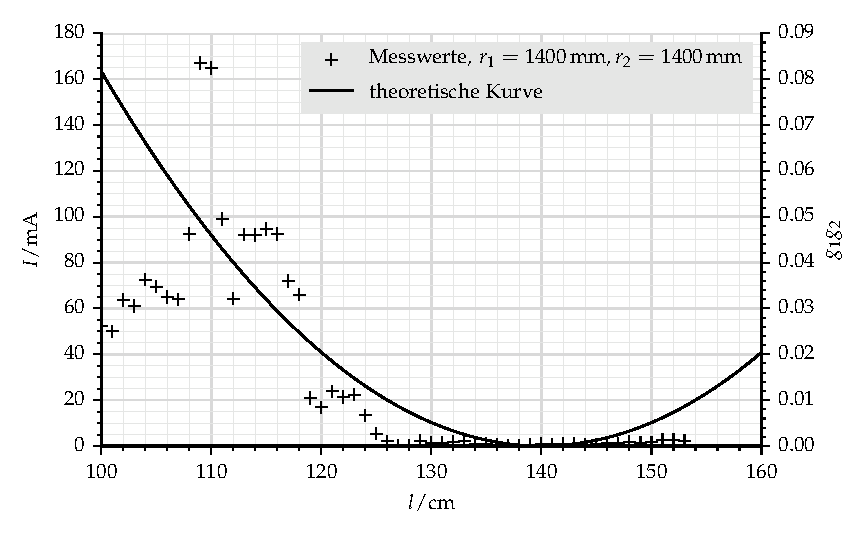
\includegraphics{bilder/fig_S1.pdf}
	\caption{Darstellung der gemessenen Diodenströme I in Abhängigkeit der
	Resonatorabstände l für den Resonator mit den Spiegelradien
	$r_1 = \SI{1400}{\milli\meter}$ und $r_2 = \SI{1400}{\milli\meter}$. Zudem
	ist die theoretische Kurve $g_1g_2$ zur Überprüfung der Stabilitätsbedingung
	eingetragen.}
	\label{fig:S1}
\end{figure}

\clearpage
\begin{SCtable}
	\centering
	\begin{tabular}{cc|cc|cc}
		\midrule
		\midrule
		$l/\si{\cm}$ & $I/\si{\mA}$ & $l/\si{\cm}$ & $I/\si{\mA}$ &
		$l/\si{\cm}$ & $I/\si{\mA}$ \\
		\midrule
		%
    \phantom{0}90         & \phantom{0}88.9       & 103                   & 48.9                  & 172                   & \phantom{0}9.4        \\
    \phantom{0}91         & \phantom{0}69.4       & 104                   & 28.0                  & 170                   & 14.1                  \\
    \phantom{0}92         & 101.9                 & 105                   & 16.1                  & 168                   & \phantom{0}8.8        \\
    \phantom{0}93         & \phantom{0}97.9       & 106                   & \phantom{0}9.3        & 166                   & \phantom{0}8.5        \\
    \phantom{0}94         & \phantom{0}87.9       & 107                   & \phantom{0}7.0        & 164                   & \phantom{0}4.9        \\
    \phantom{0}95         & \phantom{0}80.4       & 108                   & \phantom{0}4.5        & 162                   & \phantom{0}4.0        \\
    \phantom{0}96         & \phantom{0}79.5       & 109                   & \phantom{0}0.6        & 160                   & \phantom{0}5.3        \\
    \phantom{0}97         & 117.1                 & 110                   & \phantom{0}0.6        & 158                   & \phantom{0}4.0        \\
    \phantom{0}98         & 111.3                 & 111                   & \phantom{0}0.0        & 156                   & \phantom{0}2.7        \\
    \phantom{0}99         & \phantom{0}95.7       & 180                   & 45.4                  & 154                   & \phantom{0}3.9        \\
    100                   & 124.9                 & 178                   & 43.0                  & 152                   & \phantom{0}1.5        \\
    101                   & \phantom{0}95.8       & 176                   & 15.2                  & 150                   & \phantom{0}0.4        \\
    102                   & \phantom{0}61.4       & 174                   & 14.9                  & 148                   & \phantom{0}0.0        \\

%
		\midrule
		\midrule
	\end{tabular}
	\caption{Darstellung der gemessenen Diodenströme $I$ zu den jeweiligen
		Resonatorlängen $l$ für den Resonator mit den Spiegelradien
		$r_1 = \SI{1000}{\milli\meter}$ und $r_2 = \SI{1400}{\milli\meter}$.}
	\label{tab:S2}
\end{SCtable}

\begin{figure}[h!]
	\centering
	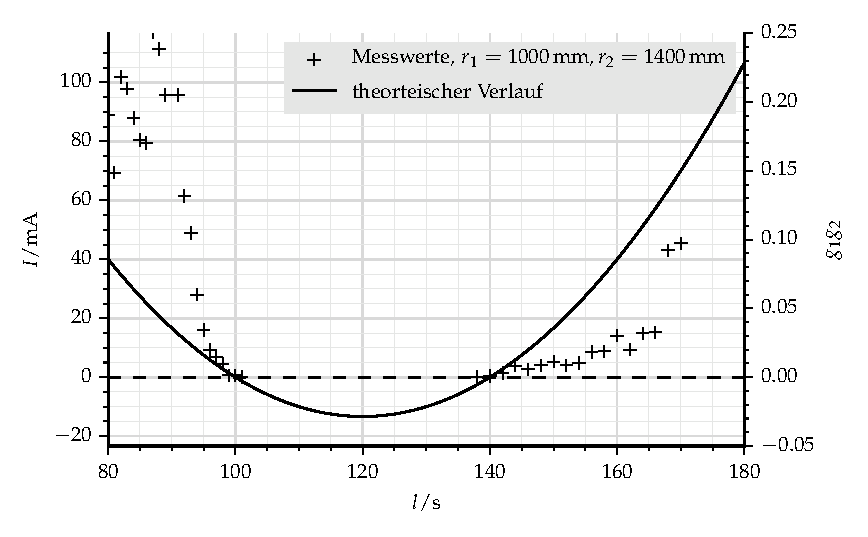
\includegraphics{bilder/fig_S2.pdf}
	\caption{Darstellung der gemessenen Diodenströme I in Abhängigkeit der
	Resonatorabstände l für den Resonator mit den Spiegelradien
	$r_1 = \SI{1000}{\milli\meter}$ und $r_2 = \SI{1400}{\milli\meter}$. Zudem
	ist die theoretische Kurve $g_1g_2$ zur Überprüfung der Stabilitätsbedingung
	eingetragen.}
	\label{fig:S2}
\end{figure}

\clearpage
% ==================================================
%	Moden
% ==================================================
\subsection{Transversale Moden}
\label{sec:Transversale_Moden}

Es wurde der Diodenstrom $I$ in Abhängigkeit des Abstandes $a$ von dem
Strahlachse gemessen, bzw es wurde nur die Einstellung Diode gemessen, sodass
die Strahlmitte nicht mit dem Nullpunkt der Skala zusammenfällt.
Die Messunge wird für den Resonator mit Spiegelradien $r_1 = r_2 =
\SI{1400}{\mm}$ durchgeführt.
Die Messwerte für die $\TEMN$-Mode befinden sich in Tabelle \ref{tab:M2} und
für die $\TEME$-Mode in Tabelle \ref{tab:M1}.
In Abbildung \ref{fig:M2} sind die Werte für die \TEMN-Mode dargestellt.
Die Werte werden entsprechend der Gleichung \eqref{eq:TEM00} mit
%
\begin{equation}
	I_{00}(r) = I_0\exp[-\left(\frac{r-r_0}{w}\right)^2]
\end{equation}
%
gefittet.
Die sich daraus ergebenden Fitparameter lauten
%
\begin{align*}
	I_0 &= \SI[parse-numbers = false]{(9.19 \pm 0.11)}{\nA} \\
	r_0 &= \SI[parse-numbers = false]{(7.99 \pm 0.05)}{\mm} \\
	w &= \SI[parse-numbers = false]{(5.44 \pm 0.08)}{\mm} ~.
\end{align*}
%
In Abbildung \ref{fig:M1} sind die Werte für die \TEME-Mode dargestellt.
Die Werte werden hier entsprechend der Gleichung \ref{eq:Feldverteilung} mit
%
\begin{equation}
	I_{10}(r) = \left( a(r-r_0)+b \right)^2 \exp[-\left(\frac{r-r_0}{w}\right)^2]
\end{equation}
%
gefittet. Die gefittet Werte lauten hier
%
\begin{align*}
	r_0 &= \SI[parse-numbers = false]{(7.92 \pm 0.09)}{\mm} \\
	w &= \SI[parse-numbers = false]{(5.07 \pm 0.08)}{\mm} \\
	a &= \SI[parse-numbers = false]{(-14.90 \pm 0.34)}{$\sqrt{\upmu\text{A}}$} \\
	b &= \SI[parse-numbers = false]{(15.7 \pm 0.9)}{$\sqrt{\upmu\text{A}}$} ~.
\end{align*}
%
\begin{table}[ht]
	\centering
	\begin{tabular}{cc|cc|cc}
		\midrule
		\midrule
		$a/\si{\mm}$ & $I/\si{\nA}$ & $a/\si{\mm}$ & $I/\si{\nA}$ &
		$a/\si{\mm}$ & $I/\si{\nA}$ \\
		\midrule
		--10.0            & 0.0037            & \phantom{0}1.0    & 1.606             & 12.0              & 5.78\phantom{0}  \\
\phantom{0}--9.0  & 0.0038            & \phantom{0}2.0    & 2.65\phantom{0}   & 13.0              & 4.0\phantom{00}  \\
\phantom{0}--8.0  & 0.0143            & \phantom{0}3.0    & 4.09\phantom{0}   & 14.0              & 2.51\phantom{0}  \\
\phantom{0}--7.0  & 0.0263            & \phantom{0}4.0    & 5.38\phantom{0}   & 15.0              & 1.49\phantom{0}  \\
\phantom{0}--6.0  & 0.0374            & \phantom{0}5.0    & 7.08\phantom{0}   & 16.0              & 0.881            \\
\phantom{0}--5.0  & 0.0537            & \phantom{0}6.0    & 7.98\phantom{0}   & 17.0              & 0.533            \\
\phantom{0}--4.0  & 0.0796            & \phantom{0}7.0    & 9.22\phantom{0}   & 18.0              & 0.223            \\
\phantom{0}--3.0  & 0.0122            & \phantom{0}8.0    & 8.94\phantom{0}   & 19.0              & 0.104            \\
\phantom{0}--2.0  & 0.232\phantom{0}  & \phantom{0}9.0    & 8.12\phantom{0}   & 20.0              & 0.05\phantom{0}  \\
\phantom{0}--1.0  & 0.441\phantom{0}  & 10.0              & 8.0\phantom{00}   & -                 & -                \\
\phantom{00}0.0   & 0.919\phantom{0}  & 11.0              & 7.28\phantom{0}   & -                 & -                \\
		\midrule
		\midrule
	\end{tabular}
	\caption{Darstellung der gemessenen Diodenströme $I$ zu den jeweiligen
		Abständen $a$ für den Resonator mit den Spiegelradien
		$r_1 = \SI{1400}{\milli\meter}$ und $r_2 = \SI{1400}{\milli\meter}$,
		wobei der Resonator in der $\text{TEM}_{00}$-Mode schwingt.}
	\label{tab:M2}
\end{table}

\begin{figure}[h!]
	\centering
	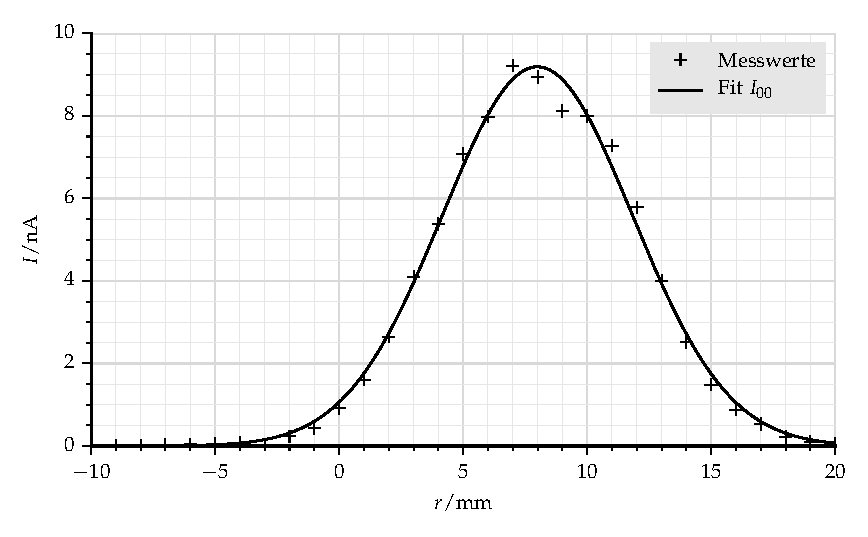
\includegraphics{bilder/fig_M2.pdf}
	\caption{Dastellung der gemessenen Diodenströme $I$ in Abhängigkeit der
	gemessenen Diodeneinstellungen $r$ senkreckt zur Strahlachse.
	Zudem ist der Fit $I_{00}(r)$ eingetragen.}
	\label{fig:M2}
\end{figure}

\clearpage
\begin{table}[hb]
	\centering
	\begin{tabular}{cc|cc|cc}
		\midrule
		\midrule
		$a/\si{\mm}$ & $I/\si{\uA}$ & $a/\si{\mm}$ & $I/\si{\uA}$ &
		$a/\si{\mm}$ & $I/\si{\uA}$ \\
		\midrule
		--10\phantom{.}   & \phantom{000}4.55 & \phantom{0}2\phantom{.} & 2600.00           & 14\phantom{.}     & 1244.00          \\
\phantom{0}--9\phantom{.} & \phantom{000}3.15 & \phantom{0}3\phantom{.} & 3220.00           & 15\phantom{.}     & 1200.00          \\
\phantom{0}--8\phantom{.} & \phantom{000}3.30 & \phantom{0}4\phantom{.} & 3300.00           & 16\phantom{.}     & \phantom{0}972.00\\
\phantom{0}--7\phantom{.} & \phantom{00}12.46 & \phantom{0}5\phantom{.} & 2640.00           & 17\phantom{.}     & \phantom{0}816.00\\
\phantom{0}--6\phantom{.} & \phantom{00}22.70 & \phantom{0}6\phantom{.} & 1580.00           & 18\phantom{.}     & \phantom{0}516.00\\
\phantom{0}--5\phantom{.} & \phantom{00}36.30 & \phantom{0}7\phantom{.} & \phantom{0}440.00 & 19\phantom{.}     & \phantom{0}318.00\\
\phantom{0}--4\phantom{.} & \phantom{0}100.00 & \phantom{0}8\phantom{.} & \phantom{00}74.00 & 20\phantom{.}     & \phantom{0}134.00\\
\phantom{0}--3\phantom{.} & \phantom{0}250.00 & \phantom{0}9\phantom{.} & \phantom{0}150.00 & 21\phantom{.}     & \phantom{00}38.00\\
\phantom{0}--2\phantom{.} & \phantom{0}570.00 & 10\phantom{.}     & \phantom{0}465.00 & 22\phantom{.}     & \phantom{00}18.00\\
\phantom{0}--1\phantom{.} & \phantom{0}928.00 & 11\phantom{.}     & \phantom{0}670.00 & 23\phantom{.}     & \phantom{00}12.50\\
\phantom{00}0\phantom{.} & 1434.00           & 12\phantom{.}     & \phantom{0}880.00 & 24\phantom{.}     & \phantom{000}3.95\\
\phantom{00}1\phantom{.} & 2200.00           & 13\phantom{.}     & 1058.00           & 25\phantom{.}     & \phantom{000}0.99\\
		\midrule
		\midrule
	\end{tabular}
	\caption{Darstellung der gemessenen Diodenströme $I$ zu den jeweiligen
		Abständen $a$ für den Resonator mit den Spiegelradien
		$r_1 = \SI{1400}{\milli\meter}$ und $r_2 = \SI{1400}{\milli\meter}$,
		wobei der Resonator in der $\text{TEM}_{10}$-Mode schwingt.}
	\label{tab:M1}
\end{table}

\begin{figure}[h!]
	\centering
	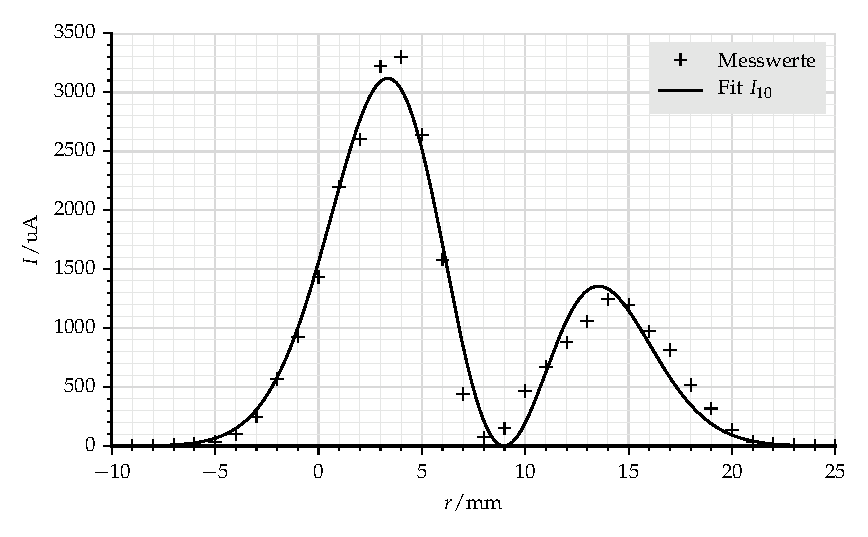
\includegraphics{bilder/fig_M1.pdf}
	\caption{Dastellung der gemessenen Diodenströme $I$ in Abhängigkeit der
	gemessenen Diodeneinstellungen $r$ senkreckt zur Strahlachse.
	Zudem ist der Fit $I_{10}(r)$ eingetragen.}
	\label{fig:M1}
\end{figure}

\clearpage
% ==================================================
%	Polarisation
% ==================================================
\subsection{Polarisation}
\label{sec:Polarisation}

In Tabelle \ref{tab:P} sind die aufgenommenen Diodenströme zu den jeweiligen
Einstellungen des Polarisationsfilters dargestellt.
In Abbildung \ref{fig:P} sind diese Werte graphisch dargestellt.
Zudem ist darin ein Fit dieser Werte mit der Funktion
%
\begin{equation}
	I_\text{P}(\varphi) = A \sin^2\left(
		\frac{\uppi}{\SI{180}{\degree}} \varphi - \varphi_0
		\right)
\end{equation}
%
eingetragen.
Die Parameter des Fits lauten hier
%
\begin{align}
	A &= \SI[parse-numbers = false]{(53.5 \pm 2.0)}{\nA} \\
	\varphi_0 &= \SI[parse-numbers = false]{(14.861 \pm 0.032)}{\degree} ~.
\end{align}

\begin{table}[hb]
	\centering
	\begin{tabular}{cc|cc|cc}
		\midrule
		\midrule
		$\varphi/\si{\degree}$ & $I/\si{\uA}$ &
		$\varphi/\si{\degree}$ & $I/\si{\uA}$ &
		$\varphi/\si{\degree}$ & $I/\si{\uA}$ \\
		\midrule
		%
    \phantom{00}0         & 24.70                 & 120                   & \phantom{0}3.32       & 240                   & 47.90                 \\
    \phantom{0}10         & 27.80                 & 130                   & \phantom{0}0.23       & 250                   & 41.80                 \\
    \phantom{0}20         & 31.00                 & 140                   & \phantom{0}0.57       & 260                   & 30.00                 \\
    \phantom{0}30         & 42.50                 & 150                   & \phantom{0}4.25       & 270                   & 17.00                 \\
    \phantom{0}40         & 46.60                 & 160                   & 16.99                 & 280                   & 12.90                 \\
    \phantom{0}50         & 50.80                 & 170                   & 27.80                 & 290                   & \phantom{0}6.20       \\
    \phantom{0}60         & 40.60                 & 180                   & 39.80                 & 300                   & \phantom{0}1.86       \\
    \phantom{0}70         & 33.90                 & 190                   & 52.90                 & 310                   & \phantom{0}0.63       \\
    \phantom{0}80         & 37.70                 & 200                   & 56.70                 & 320                   & \phantom{0}0.73       \\
    \phantom{0}90         & 35.20                 & 210                   & 56.60                 & 330                   & \phantom{0}3.60       \\
    100                   & 21.60                 & 220                   & 72.60                 & 340                   & \phantom{0}8.58       \\
    110                   & 10.93                 & 230                   & 50.50                 & 350                   & 15.44                 \\

%
		\midrule
		\midrule
	\end{tabular}
	\caption{Darstellung der gemessenen Diodenströme $I$ zu den jeweiligen
		Einstellung der Polarisationsfilters $\varphi$
		für den Resonator mit den Spiegelradien
		$r_1 = \SI{1400}{\milli\meter}$ und $r_2 = \SI{1400}{\milli\meter}$.}
	\label{tab:P}
\end{table}

\begin{figure}[h!]
	\centering
	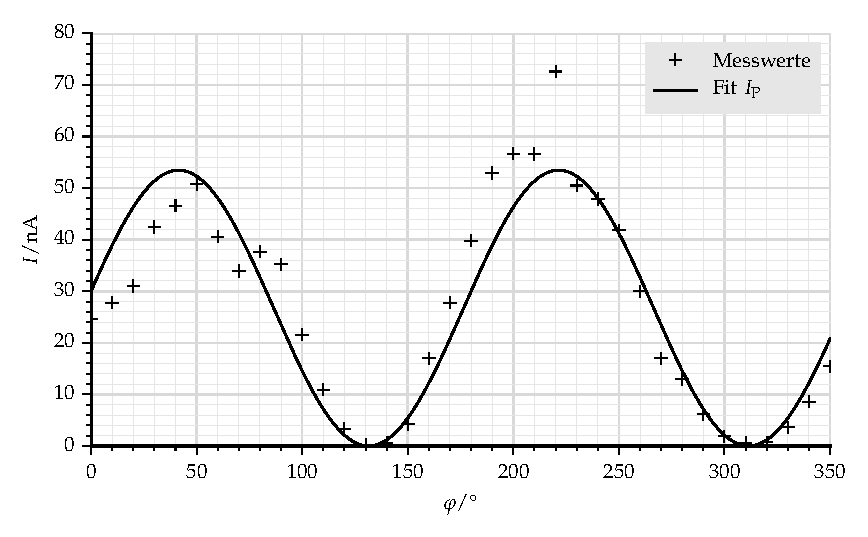
\includegraphics{bilder/fig_P.pdf}
	\caption{Darstellung der gemessenen Diodenströme $I$ in Abhängigkeit des
	eingestellten Winkels $\varphi$ am Polarisationsfilter.
	Zudem ist der Fit $I_\text{P}$ eingetragen.}
	\label{fig:P}
\end{figure}

\clearpage
% ==================================================
%	Gitter
% ==================================================
\subsection{Besimmung der Wellenlänge des HeNe-Lasers}
\label{sec:Gitter}

Die Wellenlänge $\lambda$ des HeNe-Lasers lässt sich aus
%
\begin{equation}
	\lambda = \frac{g \sin(\varphi_n)}{n}
	\label{eq:lambda_phi}
\end{equation}
%
bestimmen, wobei $n$ die Ordung des Beugungsmaximums, $g$ die Gitterkonstante
und $\varphi_n$ der Beugungswinkel des $n$-ten Beugungsmaximums zum Maximum der
nullten Ordnung ist.
Der Beugungswinkel $\varphi_n$ ergibt sich hierbei aus
%
\begin{equation}
	\varphi_n = \arctan(\frac{a}{L}) ~,
	\label{eq:Winkelbeziehung}
\end{equation}
%
wobei $L$ der Abstand vom Gitter zum Schirm und $a$ der Abstand vom
$n$-ten Beugungsmaximum zum Beugungsmaximum der nullten Ordnung ist.
Einsetzen dieser Beziehung in \eqref{eq:lambda_phi} ergibt schließlich
%
\begin{equation}
	% \tcboxmath[skin=enhanced, arc=0pt, frame hidden]{
		\lambda = \frac{g}{n \sqrt{1 + \left(\frac{L}{a}\right)^2}} ~.
		\label{eq:lambda_komplett}
\end{equation}
%
In Tabelle \ref{tab:G} sind die gemessenen Werte der Beugungsmaxima
dargestellt. Mit Hilfe dieser Werte und der Gleichung
\eqref{eq:lambda_komplett} werden der Mittelwert und die Standardabweichung
bestimmt.
Die Berechnung liefert schließlich für die Wellenlänge des HeNe-Lasers einen
Wert von
%
\begin{equation}
	\lambda = \SI[parse-numbers = false]{(622.3 \pm 25.9)}{\nano\meter} ~.
	\label{eq:l_ergebnis}
\end{equation}
%
\begin{table}[hb]
	\centering
	\begin{tabular}{ccc|ccc}
		\midrule
		\midrule
		$n$ & $a_r/\si{\cm}$ & $a_l/\si{\cm}$ &
		$n$ & $a_r/\si{\cm}$ & $a_l/\si{\cm}$ \\
		\midrule
		\SI[parse-numbers = false]{-0.7009 \pm 0.0025}{}
		\midrule
		\midrule
	\end{tabular}
	\caption{Darstellung der Abstände $a_r$ und $a_l$ der Beugungsmaxima der
		jeweiligen Ordnung $n$ rechts
		und links von der nullten Ordnung aus gemessen.}
	\label{tab:G}
\end{table}
